\documentclass[10pt,letterpaper,english,hidelinks]{amsart}

\usepackage{amsmath}
\usepackage{amssymb}
\usepackage{amsthm}
\usepackage{fancyhdr}
\usepackage{graphicx}
\usepackage{pgfplots}
\usepackage{tikz}
\usepackage{datetime2}
\usepackage{natbib}
\usepackage[unicode]{hyperref}
\usepackage{mathtools}
\mathtoolsset{showonlyrefs}

\usetikzlibrary{fadings}
\usetikzlibrary{patterns}
\usetikzlibrary{shadows.blur}
\usetikzlibrary{arrows}
\usetikzlibrary{decorations.markings}
\usetikzlibrary{positioning}
\usetikzlibrary{calc}
\usetikzlibrary{math}

\pgfplotsset{compat=1.16}

\DTMnewdatestyle{mydateformat}{%
  \renewcommand{\DTMdisplaydate}[4]{%
    \number##1\ % year
    \DTMenglishmonthname{##2}\ % Month
    \number##3% day
  }%
  \renewcommand{\DTMDisplaydate}{\DTMdisplaydate}%
}
\DTMsetdatestyle{mydateformat}

% text dimensions
\setlength{\textwidth}{6.5in}
\setlength{\textheight}{9in}

% adjust top margins
\setlength{\topmargin}{0in}
\setlength{\voffset}{-30pt}
\setlength{\headheight}{12pt}

% no room for notes on the side
\setlength{\oddsidemargin}{0in}
\setlength{\evensidemargin}{0in}
\setlength{\marginparwidth}{0in}

% space between paragraphs and lines
\setlength{\parskip}{5pt}
\linespread{1.05} % for final submission
% \linespread{2} % for editing drafts

% Hyphenation
\numberwithin{equation}{section}
\hyphenation{semi-stable}

% Numbering for Theorems, Lemmas, etc.
\theoremstyle{plain}
\newtheorem{theorem}{Theorem}[section]
\newtheorem{corollary}[theorem]{Corollary}
\newtheorem{lemma}[theorem]{Lemma}
\newtheorem{conjecture}[theorem]{Conjecture}
\theoremstyle{definition}
\newtheorem{definition}[theorem]{Definition}
\newtheorem{example}[theorem]{Example}
\newtheorem{remark}[theorem]{Remark}
\numberwithin{equation}{section}

% Header Definitions
\fancyhead[L]{\nouppercase{\rightmark}}
\fancyhead[R]{\nouppercase{\leftmark}}

\pagestyle{fancy}

\newcommand{\cech}{\v{C}ech }
\DeclareMathOperator{\Cech}{\textrm{\v{C}ech}}
\DeclareMathOperator{\Ima}{Im}
\DeclareMathOperator{\Ker}{Ker}
\DeclareMathOperator{\nul}{Null}
\DeclareMathOperator{\boundary}{\partial}
\newcommand*{\Z}{\mathbb{Z}}
\newcommand{\bigslant}[2]{%
  \mathchoice
  {{\raisebox{.2em}{$#1$}\left/\raisebox{-.2em}{$#2$}\right.}}
  {{\raisebox{0em}{$#1$}\left/\raisebox{0em}{$#2$}\right.}}
  {{\raisebox{0em}{$#1$}\left/\raisebox{0em}{$#2$}\right.}}
  {{\raisebox{0em}{$#1$}\left/\raisebox{0em}{$#2$}\right.}}
}
\newcommand{\cross}{\times}
\newcommand{\normalsubgroup}{\triangleleft}
\newcommand{\figref}[1]{[Fig. \ref{#1}]}
\newcommand{\subfigref}[2]{[Fig. \ref{#1}, #2]}
\newcommand{\red}[1]{{\color{red} #1}}
\newcommand{\lightgray}[1]{{\color{lightgray} #1}}


\title[Persistent Homology]{Persistent Homology: Computations and Applications}
\author{Stephen Ermshar}
\address{Department of Mathematics, Walla Walla University, College Place, WA 99324}
\date{\DTMDisplaydate{2020}{5}{29}{}} % pre-final draft due
\thanks{Advisor: Dr. John Foster}

% for keeping track of printed drafts, adds date and time to every page
\thanks{\tiny{\DTMtoday, \DTMcurrenttime}}
\rfoot{\hfill\newline\tiny{\DTMtoday, \DTMcurrenttime}}


\begin{document}

\begin{abstract}
    % <300 word abstract.
    Persistent Homology is a method for understanding a numerical multi dimensional data set by observing certain features of shapes generated by the data.
    These features of interest are holes, and can provide clues for how the data is connected or where data may be missing.
    Homology is the study of these holes, and Persistent Homology is a natural application of this topic to data sets.
    This paper will provide an introduction to Simplicial Homology and how it can be applied to a data set.
\end{abstract}
\maketitle

\section{Introduction}

Persistent homology is a tool for understanding the shape of a data set.
If a data set is a collection of points in two dimensional space, then it can be graphed in a plane.
We can easily look at the graph and see whether the data clumps together in certain places, or if it forms more interesting shapes, like loops.
We can graph data from one and three dimensions as well, but with dimensions four and higher we are no longer able to visualize the data in a traditional scatter plot.

\begin{figure}[h]
    \centering
    \scalebox{0.75}{\tikzset{
pattern size/.store in=\mcSize,
pattern size = 5pt,
pattern thickness/.store in=\mcThickness,
pattern thickness = 0.3pt,
pattern radius/.store in=\mcRadius,
pattern radius = 1pt}
\makeatletter
\pgfutil@ifundefined{pgf@pattern@name@_iy1rqtf17}{
\pgfdeclarepatternformonly[\mcThickness,\mcSize]{_iy1rqtf17}
{\pgfqpoint{0pt}{0pt}}
{\pgfpoint{\mcSize+\mcThickness}{\mcSize+\mcThickness}}
{\pgfpoint{\mcSize}{\mcSize}}
{
\pgfsetcolor{\tikz@pattern@color}
\pgfsetlinewidth{\mcThickness}
\pgfpathmoveto{\pgfqpoint{0pt}{0pt}}
\pgfpathlineto{\pgfpoint{\mcSize+\mcThickness}{\mcSize+\mcThickness}}
\pgfusepath{stroke}
}}
\makeatother

% https://ipfs-sec.stackexchange.cloudflare-ipfs.com/tex/A/question/6135.html
\tikzset{every picture/.style={line width=0.75pt, opacity=0}} %set default line width to 0.75pt
\tikzset{onslide/.code args={<#1>#2}{%
    \only<#1>{\pgfkeysalso{#2}} % \pgfkeysalso doesn't change the path
}}

\begin{tikzpicture}[x=0.75pt,y=0.75pt,yscale=-1,xscale=1]

    \def\points{
        (240,312),
        (230,238),
        (282,164),
        (300,320),
        (348,180),
        (348,336),
        (398,262),
        (406,322)
    }

    % \def\points{
    %     (134,150),
    %     (166,136),
    %     (118,298),
    %     (178,312),
    %     (114,222),
    %     (232,342),
    %     (322,232),
    %     (316,324),
    %     (280,342),
    %     (504,284),
    %     (418,350),
    %     (388,184),
    %     (292,126),
    %     (324,172),
    %     (234,108),
    %     (246,154),
    %     (162,192),
    %     (458,210),
    %     (362,348)
    % }

    \foreach \r [count=\ri from 2] in {40, 50, 60, 85}{
        \foreach \p in \points{
            \draw
                [color={rgb, 255:red, 165; green, 232; blue, 255}]
                [fill={rgb, 255:red, 165; green, 232; blue, 255}]
                [onslide=<{\ri}>{opacity=1}]
                [line width=0]
                \p circle
                [radius=\r];
        }
        \foreach \a [count=\ai] in \points{
            \foreach \b [count=\bi] in \points{
                \path \a;
                \pgfgetlastxy{\ax}{\ay}
                \path \b;
                \pgfgetlastxy{\bx}{\by}
                \pgfmathsetmacro\thresh{2*\r}
                % The 23 on the following line is there because
                % this calculation connected some vertices before the
                % circles drawn underneath overlapped. the adjustment
                % doesn't appear to make the graph incorrect and forces
                % the vertices to wait longer before connecting, though
                % it is concerning.
                \pgfmathsetmacro\dist{veclen(\ax-\bx,\ay-\by)+23}
                \ifnum\ai<\bi
                    \ifdim\dist pt<\thresh pt
                        \draw
                        [onslide=<{\ri}>{opacity=1}]
                        \a -- \b;
                    \fi
                \fi

            }
        }
    }

    % Vertices go at the bottom so they're on top of the rest
    \foreach \p [count=\pi] in \points{
        \draw
            [black, fill=black]
            [opacity=1]
            \p circle
            [radius= 3.35];
        % \draw % mark nodes for debugging
        %     [opacity=1]
        %     \x+(10,10) node {\(\pi\)};
    }

\end{tikzpicture}
}
    \caption{}
    \label{fig:persistence-demo-r25}
\end{figure}

To get an idea of the shape formed by a data set we connect nearby points.
A threshold radius can be used to determine whether points are close enough to be considered related.
With the resulting graph-like structure we can apply tools from homology to find holes like the two shown in figure \ref{fig:persistence-demo-r25}.
Homology will help us find higher dimensional analogues of these holes as well, such as voids, which are the space inside an enclosed surface \red{(cite?)}.

The graph-like structure, which is called a simplicial complex, will change depending on the value of the radius.
If the radius is small enough then no points will be connected, and if it is large enough then all the points will be connected.
Between these two extremes more interesting simplicial complexes result.
As the radius increases, holes will form and points begin to connect.
Eventually as more points connect those holes will get filled in.
The holes that persist over a wide range of radius values are considered to be the more significant features of the shape.

In section \ref{sec:homology} we'll formalize the simplicial complex and its building blocks.
Then, given an existing simplicial complex we'll solidify the concept with an example computation for finding a hole.
As we move on to persistent homology in section \ref{sec:persistent-homology}, we'll introduce the cech complex, which is used to build a simplicial complex given a data set and a radius.
Having calculated the homology for the cech complex along a range of scales we'll look at two methods for visualizing the results, and \red{might} look at the stability theorem, which will ensure that the results are reliable.
Finally, in section \ref{sec:applications} we \red{might} explore applications for persistent homology.

\section{Homology}\label{sec:homology}

\subsection{Simplicial Homology}\label{sec:simplicial-homology}

The basic building block of a simplicial complex is an \(n\)-simplex. % are simplices
An \(n\)-simplex generalizes the triangle to \(n\) dimensions by associating \(n+1\) vertices with each other in an ordered tuple.
For instance, a point is a 0-simplex, an edge a 1-simplex, a triangle a 2-simplex, a tetrahedron a 3-simplex, and so on \figref{fig:basic-simplices}.

\begin{figure}
    \tikzset{every picture/.style={line width=0.75pt}} %set default line width to 0.75pt

\begin{tikzpicture}[x=0.75pt,y=0.75pt,yscale=-1,xscale=1]

\coordinate (01) at (77,72);
\coordinate (11) at (147,71);
\coordinate (12) at (179,59.5);
\coordinate (21) at (233.21,91.12);
\coordinate (22) at (276.15,74.49);
\coordinate (23) at (239.92,44.11);
\coordinate (31) at (320,65.5);
\coordinate (32) at (345,30.5);
\coordinate (33) at (369,65.5);
\coordinate (34) at (342,90.5);

% 0 Simplex
\draw   [black, fill=black] (01) circle [radius= 3.35] ;

% 1 Simplex
\draw   [black, fill=black] (11) circle [radius= 3.35] ;
\draw   [black, fill=black] (12) circle [radius= 3.35] ;
\draw   (11) -- (12) ;

% 2 Simplex
\draw   [black, fill=lightgray] (21) -- (22) -- (23) -- cycle   ;
\draw   [black, fill=black] (21) circle [radius= 3.35] ;
\draw   [black, fill=black] (22) circle [radius= 3.35] ;
\draw   [black, fill=black] (23) circle [radius= 3.35] ;

% 3 Simplex
\draw   [black, fill=lightgray] (31) -- (32) -- (34) -- cycle   ;
\draw   [black, fill=gray]      (32) -- (33) -- (34) -- cycle   ;
\draw   [dash pattern={on 4.5pt off 4.5pt}]  (31) -- (33) ;
\draw   [black, fill=black] (31) circle [radius= 3.35] ;
\draw   [black, fill=black] (32) circle [radius= 3.35] ;
\draw   [black, fill=black] (33) circle [radius= 3.35] ;
\draw   [black, fill=black] (34) circle [radius= 3.35] ;

% Straight Arrow
\draw [shift={(163,65.25)}, rotate = 520.23] [fill={rgb, 255:red, 0; green, 0; blue, 0 }  ][line width=0.08]  [draw opacity=0] (8.93,-4.29) -- (0,0) -- (8.93,4.29) -- cycle    ;

% Circle Arrow
\draw  [draw opacity=0] (255.97,69.08) .. controls (255.99,69.3) and (256,69.52) .. (256,69.75) .. controls (256,73.48) and (252.87,76.5) .. (249,76.5) .. controls (245.13,76.5) and (242,73.48) .. (242,69.75) .. controls (242,66.02) and (245.13,63) .. (249,63) .. controls (249.81,63) and (250.59,63.13) .. (251.32,63.38) -- (249,69.75) -- cycle ; \draw   (255.97,69.08) .. controls (255.99,69.3) and (256,69.52) .. (256,69.75) .. controls (256,73.48) and (252.87,76.5) .. (249,76.5) .. controls (245.13,76.5) and (242,73.48) .. (242,69.75) .. controls (242,66.02) and (245.13,63) .. (249,63) .. controls (249.81,63) and (250.59,63.13) .. (251.32,63.38) ;
\draw  [fill={rgb, 255:red, 0; green, 0; blue, 0 }  ,fill opacity=1 ] (253.25,70.52) -- (255.25,65.85) -- (258.47,69.77) ;


% Caption Labels
\draw (78,116)   node   [align=left] {0-simplex};
\draw (166,117)  node   [align=left] {1-simplex};
\draw (256,117)  node   [align=left] {2-simplex};
\draw (347,116)  node   [align=left] {3-simplex};
\draw (78,136)   node   [align=left] {(1)};
\draw (166,137)  node   [align=left] {(1,2)};
\draw (256,137)  node   [align=left] {(1,2,3)};
\draw (347,136)  node   [align=left] {(1,2,3,4)};

% Vertex Labels
\draw (01)+(-10,5)  node   [align=left] {1};
\draw (11)+(-10,5)  node   [align=left] {1};
\draw (12)+(10,5)   node   [align=left] {2};
\draw (21)+(-10,5)  node   [align=left] {1};
\draw (22)+(10,5)   node   [align=left] {2};
\draw (23)+(-10,5)  node   [align=left] {3};
\draw (31)+(-10,5)  node   [align=left] {1};
\draw (32)+(10,0)   node   [align=left] {2};
\draw (33)+(10,5)   node   [align=left] {3};
\draw (34)+(-10,5)  node   [align=left] {4};




\end{tikzpicture}

    \caption{}
    \label{fig:basic-simplices}
\end{figure}

A simplicial complex will be a collection of simplices.
For a simplex to be considered part of a simplicial complex it will need to have been built up from lower dimensional simplices.
A triangle includes its three edges and three vertices, so if a triangle is included in a simplicial complex we will require that all of its edges and vertices are also included in the complex.

\begin{definition}\label{def:simplicial-complex}
    A \textbf{Simplicial Complex} is a finite collection of finite sets such that every subset of every element in the collection is also an element in the collection. \cite{wagner}
\end{definition}

This will be a useful property because when we study the homology of the complex we will be comparing the boundaries of its \(n\)-simplices, which are \((n-1)\)-simplices, to other \((n-1)\)-simplices in the complex.

Homology will be calculated by finding all the loops of \((n-1)\)-simplices, and ignoring any loops of \((n-1)\)-simplices around \(n\)-simplices, leaving only loops of \((n-1)\)-simplices that surround empty space that could be filled with \(n\)-simplices.
These remaining loops are what we intuitively call holes.

A path of \(n\)-simplices can just be thought of as a list of \(n\)-simplices; this makes intuitive sense for 1-simplices, where a list of edges describes a 1-dimensional path through a complex, but still works for larger values of \(n\).
For instance, a closed path of 2-simplices around a tetrahedron consists of its four faces.

\subsection{Computations}

In practice we can think of paths of \(n\)-simplices as linear combinations of \(n\)-simplices.
Figure \ref{fig:example-cech} shows a complex \(C = \{ (1,2,3), (1,2), (1,3), (2,3), (2,4), (3,4), (1), (2), (3), (4) \}\) where \(\ell_1\) is the closed path of 1-simplices around the outside of the complex and \(\ell_2\) is the closed path of 1-simplices around the 2-simplex \((1,2,3)\).
When we write down a simplex we always write its elements in increasing order by label.
Note that the negative signs in \(\ell_1\) and \(\ell_2\) correspond to traveling backwards along an edge.
This convention allows us to give each simplex an orientation, so that when we add a simplex to a copy of itself with an opposite orientation they will cancel out.
If we were to add \(\ell_1\) and \(\ell_2\), the simplices \((1, 3)\) and \((1, 2)\) would cancel out, leaving the element \((3, 4) - (2, 4) + (2, 3)\), which corresponds to the loop around the hole.

A closed path of \((n-1)\)-simplices around an \(n\)-simplex will represent the boundary of the \(n\)-simplex. We can also add \(n\)-simplices together and take the boundary of the resulting element. To more formally describe boundaries of \(n\)-simplices we define the boundary homomorphism, which maps elements from the group of \(n\)-simplices to elements in the group of \((n-1)\)-simplices.

\begin{definition}\label{def:boundary-homomorphism}
    The \(n\textsuperscript{th}\) \textbf{Boundary Homomorphism} \(\boundary_n : C_n \to C_{n-1}\) is
    \[
        \boundary_n (v_1,\dots , v_{n+1}) = \sum_{i=1}^{n+1} (-1)^{i+1}
        (v_1,\dots, v_{i-1}, v_{i+1}, \dots, v_{n+1})
        .
    \]
    \cite{hatcher}
\end{definition}

\red{(Is there a nice way to explain the alternating sign in def \ref{def:boundary-homomorphism}?)}

\begin{example}
    If the example complex in figure \ref{fig:example-cech} were to include the triangle \((2,3,4)\), then we could combine the two triangles and would expect their boundary to be the loop around the outside of the complex, \(\ell_1\). The triangle \((2,3,4)\) has clockwise orientation, while \((1,2,3)\) has counterclockwise orientation. If we were to give them both the same orientation and then add them, then the simplex \((2,3)\) in their boundaries would cancel, resulting in \(\ell_1\) as expected.
\end{example}

The boundary homomorphism will help us find all boundaries of \(n\)-simplices in a complex. With the help of theorem \ref{thm:zero-boundary} we'll also be able to find all closed paths of \(n\)-simplices in a complex.

\begin{theorem}\label{thm:zero-boundary}
    The composition of two boundary homomorphisms is zero. For any element \(c\) in the group of \((n+1)\)-simplices
    \begin{align*}
        \boundary_{n} \Big( \boundary_{n+1} (c) \Big) = 0
        .
    \end{align*}
    \red{(cite?)}
\end{theorem}

The boundary of a boundary is always zero;
Any element from the group of \(n\)-simplices that is a boundary is in the kernel of the \(n\textsuperscript{th}\) boundary homomorphism, that is, \(\Ima(\boundary_{n+1}) \subseteq \Ker(\boundary_n))\).
The kernel of a boundary homomorphism will represent all closed paths in a complex \red{(It'd be nice to have a good explanation of this sentence.)}.

% replace this paragraph

Since we're not concerned with the order in which simplices are added, the groups of simplices are abelian, so \(\Ima(\boundary_{n+1}) \normalsubgroup \Ker(\boundary_{n})  \).

% replace with image is normal subgroup.

\begin{definition}\label{def:nth-homology-group}
    The \textbf{n-th Homology Group} is \[H_n = \bigslant{\Ker(\boundary_n)}{\Ima(\boundary_{n+1})}.\]
    \cite{fraleigha}
\end{definition}

This is the group of closed paths, or cycles, modded out by cycles around simplices. The result is just the cycles not surrounding simplices. We will demonstrate this computation to find the first homology group of the complex shown in figure \ref{fig:example-cech}.

\begin{example}

    \begin{figure}
        \centering
        \begin{minipage}{.5\textwidth}
            \centering
            \tikzset{
pattern size/.store in=\mcSize,
pattern size = 5pt,
pattern thickness/.store in=\mcThickness,
pattern thickness = 0.3pt,
pattern radius/.store in=\mcRadius,
pattern radius = 1pt}
\makeatletter
\pgfutil@ifundefined{pgf@pattern@name@_iy1rqtf17}{
\pgfdeclarepatternformonly[\mcThickness,\mcSize]{_iy1rqtf17}
{\pgfqpoint{0pt}{0pt}}
{\pgfpoint{\mcSize+\mcThickness}{\mcSize+\mcThickness}}
{\pgfpoint{\mcSize}{\mcSize}}
{
\pgfsetcolor{\tikz@pattern@color}
\pgfsetlinewidth{\mcThickness}
\pgfpathmoveto{\pgfqpoint{0pt}{0pt}}
\pgfpathlineto{\pgfpoint{\mcSize+\mcThickness}{\mcSize+\mcThickness}}
\pgfusepath{stroke}
}}
\makeatother
\tikzset{every picture/.style={line width=0.75pt}} %set default line width to 0.75pt

\begin{tikzpicture}[x=0.75pt,y=0.75pt,yscale=-1,xscale=1]
%uncomment if require: \path (0,95); %set diagram left start at 0, and has height of 95

\draw [shift={(163,23.5)}, rotate = 99.21] [color={rgb, 255:red, 165; green, 232; blue, 255}  ][fill={rgb, 255:red, 165; green, 232; blue, 255 }  ][line width=0]      (0, 0) circle [x radius= 20, y radius= 20]   ;
\draw [shift={(135,40)}, rotate = 349.29] [color={rgb, 255:red, 165; green, 232; blue, 255}  ][fill={rgb, 255:red, 165; green, 232; blue, 255 }  ][line width=0]      (0, 0) circle [x radius= 20, y radius= 20]   ;
\draw [shift={(13,61)}, rotate = 312.63] [color={rgb, 255:red, 165; green, 232; blue, 255}  ][fill={rgb, 255:red, 165; green, 232; blue, 255 }  ][line width=0]      (0, 0) circle [x radius= 20, y radius= 20]   ;
\draw [shift={(56,17)}, rotate = 0] [color={rgb, 255:red, 165; green, 232; blue, 255}  ][fill={rgb, 255:red, 165; green, 232; blue, 255 }  ][line width=0]      (0, 0) circle [x radius= 20, y radius= 20]   ;
\draw [shift={(69,54)}, rotate = 329.74] [color={rgb, 255:red, 165; green, 232; blue, 255}  ][fill={rgb, 255:red, 165; green, 232; blue, 255 }  ][line width=0]      (0, 0) circle [x radius= 20, y radius= 20]   ;
\draw [shift={(95,25)}, rotate = 353.99] [color={rgb, 255:red, 165; green, 232; blue, 255}  ][fill={rgb, 255:red, 165; green, 232; blue, 255 }  ][line width=0]      (0, 0) circle [x radius= 20, y radius= 20]   ;
\draw [shift={(95,25)}, rotate = 69.78] [color={rgb, 255:red, 165; green, 232; blue, 255}  ][fill={rgb, 255:red, 165; green, 232; blue, 255 }  ][line width=0]      (0, 0) circle [x radius= 20, y radius= 20]   ;
\draw [shift={(135,40)}, rotate = 314.34] [color={rgb, 255:red, 165; green, 232; blue, 255}  ][fill={rgb, 255:red, 165; green, 232; blue, 255 }  ][line width=0]      (0, 0) circle [x radius= 20, y radius= 20]   ;
\draw [shift={(157,60.5)}, rotate = 31.29] [color={rgb, 255:red, 165; green, 232; blue, 255}  ][fill={rgb, 255:red, 165; green, 232; blue, 255 }  ][line width=0]      (0, 0) circle [x radius= 20, y radius= 20]   ;
\draw [shift={(157,60.5)}, rotate = 349.29] [color={rgb, 255:red, 165; green, 232; blue, 255}  ][fill={rgb, 255:red, 165; green, 232; blue, 255 }  ][line width=0]      (0, 0) circle [x radius= 20, y radius= 20]   ;
\draw [shift={(157,60.5)}, rotate = 99.21] [color={rgb, 255:red, 165; green, 232; blue, 255}  ][fill={rgb, 255:red, 165; green, 232; blue, 255 }  ][line width=0]      (0, 0) circle [x radius= 20, y radius= 20]   ;
\draw [shift={(56,17)}, rotate = 312.63] [color={rgb, 255:red, 165; green, 232; blue, 255}  ][fill={rgb, 255:red, 165; green, 232; blue, 255 }  ][line width=0]      (0, 0) circle [x radius= 20, y radius= 20]   ;
\draw [shift={(95,25)}, rotate = 31.29] [color={rgb, 255:red, 165; green, 232; blue, 255}  ][fill={rgb, 255:red, 165; green, 232; blue, 255 }  ][line width=0]      (0, 0) circle [x radius= 20, y radius= 20]   ;
\draw [shift={(95,25)}, rotate = 0] [color={rgb, 255:red, 165; green, 232; blue, 255}  ][fill={rgb, 255:red, 165; green, 232; blue, 255 }  ][line width=0]      (0, 0) circle [x radius= 20, y radius= 20]   ;
\draw [shift={(69,54)}, rotate = 36.87] [color={rgb, 255:red, 165; green, 232; blue, 255}  ][fill={rgb, 255:red, 165; green, 232; blue, 255 }  ][line width=0]      (0, 0) circle [x radius= 20, y radius= 20]   ;
\draw [shift={(56,17)}, rotate = 36.87] [color={rgb, 255:red, 165; green, 232; blue, 255}  ][fill={rgb, 255:red, 165; green, 232; blue, 255 }  ][line width=0]      (0, 0) circle [x radius= 20, y radius= 20]   ;
\draw [shift={(95,25)}, rotate = 329.74] [color={rgb, 255:red, 165; green, 232; blue, 255}  ][fill={rgb, 255:red, 165; green, 232; blue, 255 }  ][line width=0]      (0, 0) circle [x radius= 20, y radius= 20]   ;
\draw [shift={(163,23.5)}, rotate = 353.99] [color={rgb, 255:red, 165; green, 232; blue, 255}  ][fill={rgb, 255:red, 165; green, 232; blue, 255 }  ][line width=0]      (0, 0) circle [x radius= 20, y radius= 20]   ;
\draw [shift={(135,40)}, rotate = 69.78] [color={rgb, 255:red, 165; green, 232; blue, 255}  ][fill={rgb, 255:red, 165; green, 232; blue, 255 }  ][line width=0]      (0, 0) circle [x radius= 20, y radius= 20]   ;
\draw [shift={(163,23.5)}, rotate = 314.34] [color={rgb, 255:red, 165; green, 232; blue, 255}  ][fill={rgb, 255:red, 165; green, 232; blue, 255 }  ][line width=0]      (0, 0) circle [x radius= 20, y radius= 20]   ;
\draw [shift={(255, 50)}, rotate = 314.34] [color={rgb, 255:red, 165; green, 232; blue, 255}  ][fill={rgb, 255:red, 165; green, 232; blue, 255 }  ][line width=0]      (0, 0) circle [x radius= 20, y radius= 20]   ;

%Straight Lines [id:da20686486428426965] (1-2)
% \draw    (13,61) -- (56,17) ;
\draw [shift={(56,17)}, rotate = 312.63] [color={rgb, 255:red, 0; green, 0; blue, 0 }  ][fill={rgb, 255:red, 0; green, 0; blue, 0 }  ][line width=0.75]      (0, 0) circle [x radius= 3.35, y radius= 3.35]   ;
\draw [shift={(13,61)}, rotate = 312.63] [color={rgb, 255:red, 0; green, 0; blue, 0 }  ][fill={rgb, 255:red, 0; green, 0; blue, 0 }  ][line width=0.75]      (0, 0) circle [x radius= 3.35, y radius= 3.35]   ;
%Straight Lines [id:da9899744043809231] (2-4)
\draw    (56,17) -- (95,25) ;
% \draw [shift={(95,25)}, rotate = 0] [color={rgb, 255:red, 0; green, 0; blue, 0 }  ][fill={rgb, 255:red, 0; green, 0; blue, 0 }  ][line width=0.75]      (0, 0) circle [x radius= 3.35, y radius= 3.35]   ;
% \draw [shift={(56,17)}, rotate = 0] [color={rgb, 255:red, 0; green, 0; blue, 0 }  ][fill={rgb, 255:red, 0; green, 0; blue, 0 }  ][line width=0.75]      (0, 0) circle [x radius= 3.35, y radius= 3.35]   ;
%Straight Lines [id:da4483952202454973] (2-3)
\draw    (56,17) -- (69,54) ;
\draw [shift={(69,54)}, rotate = 36.87] [color={rgb, 255:red, 0; green, 0; blue, 0 }  ][fill={rgb, 255:red, 0; green, 0; blue, 0 }  ][line width=0.75]      (0, 0) circle [x radius= 3.35, y radius= 3.35]   ;
\draw [shift={(56,17)}, rotate = 36.87] [color={rgb, 255:red, 0; green, 0; blue, 0 }  ][fill={rgb, 255:red, 0; green, 0; blue, 0 }  ][line width=0.75]      (0, 0) circle [x radius= 3.35, y radius= 3.35]   ;
%Straight Lines [id:da013663715151336797](3-4)
\draw    (69,54) -- (95,25) ;
\draw [shift={(95,25)}, rotate = 329.74] [color={rgb, 255:red, 0; green, 0; blue, 0 }  ][fill={rgb, 255:red, 0; green, 0; blue, 0 }  ][line width=0.75]      (0, 0) circle [x radius= 3.35, y radius= 3.35]   ;
\draw [shift={(69,54)}, rotate = 329.74] [color={rgb, 255:red, 0; green, 0; blue, 0 }  ][fill={rgb, 255:red, 0; green, 0; blue, 0 }  ][line width=0.75]      (0, 0) circle [x radius= 3.35, y radius= 3.35]   ;
%Straight Lines [id:da6445202628566384](4-7)
% \draw    (95,25) -- (163,23.5) ;
\draw [shift={(163,23.5)}, rotate = 353.99] [color={rgb, 255:red, 0; green, 0; blue, 0 }  ][fill={rgb, 255:red, 0; green, 0; blue, 0 }  ][line width=0.75]      (0, 0) circle [x radius= 3.35, y radius= 3.35]   ;
\draw [shift={(95,25)}, rotate = 353.99] [color={rgb, 255:red, 0; green, 0; blue, 0 }  ][fill={rgb, 255:red, 0; green, 0; blue, 0 }  ][line width=0.75]      (0, 0) circle [x radius= 3.35, y radius= 3.35]   ;
%Straight Lines [id:da3743946516627876] (4-5)
% \draw    (95,25) -- (135,40) ;
\draw [shift={(135,40)}, rotate = 69.78] [color={rgb, 255:red, 0; green, 0; blue, 0 }  ][fill={rgb, 255:red, 0; green, 0; blue, 0 }  ][line width=0.75]      (0, 0) circle [x radius= 3.35, y radius= 3.35]   ;
\draw [shift={(95,25)}, rotate = 69.78] [color={rgb, 255:red, 0; green, 0; blue, 0 }  ][fill={rgb, 255:red, 0; green, 0; blue, 0 }  ][line width=0.75]      (0, 0) circle [x radius= 3.35, y radius= 3.35]   ;
%Straight Lines [id:da2401873796980163] (5-7)
\draw    (135,40) -- (163,23.5) ;
\draw [shift={(163,23.5)}, rotate = 314.34] [color={rgb, 255:red, 0; green, 0; blue, 0 }  ][fill={rgb, 255:red, 0; green, 0; blue, 0 }  ][line width=0.75]      (0, 0) circle [x radius= 3.35, y radius= 3.35]   ;
\draw [shift={(135,40)}, rotate = 314.34] [color={rgb, 255:red, 0; green, 0; blue, 0 }  ][fill={rgb, 255:red, 0; green, 0; blue, 0 }  ][line width=0.75]      (0, 0) circle [x radius= 3.35, y radius= 3.35]   ;
%Straight Lines [id:da08347218855288774] (4-6)
% \draw    (95,25) -- (157,60.5) ;
\draw [shift={(157,60.5)}, rotate = 31.29] [color={rgb, 255:red, 0; green, 0; blue, 0 }  ][fill={rgb, 255:red, 0; green, 0; blue, 0 }  ][line width=0.75]      (0, 0) circle [x radius= 3.35, y radius= 3.35]   ;
\draw [shift={(95,25)}, rotate = 31.29] [color={rgb, 255:red, 0; green, 0; blue, 0 }  ][fill={rgb, 255:red, 0; green, 0; blue, 0 }  ][line width=0.75]      (0, 0) circle [x radius= 3.35, y radius= 3.35]   ;
%Straight Lines [id:da34695654406224863]
\draw    (135,40) -- (157,60.5) ;
\draw [shift={(157,60.5)}, rotate = 349.29] [color={rgb, 255:red, 0; green, 0; blue, 0 }  ][fill={rgb, 255:red, 0; green, 0; blue, 0 }  ][line width=0.75]      (0, 0) circle [x radius= 3.35, y radius= 3.35]   ;
\draw [shift={(135,40)}, rotate = 349.29] [color={rgb, 255:red, 0; green, 0; blue, 0 }  ][fill={rgb, 255:red, 0; green, 0; blue, 0 }  ][line width=0.75]      (0, 0) circle [x radius= 3.35, y radius= 3.35]   ;
%Straight Lines [id:da5097015872445443]
\draw    (163,23.5) -- (157,60.5) ;
\draw [shift={(157,60.5)}, rotate = 99.21] [color={rgb, 255:red, 0; green, 0; blue, 0 }  ][fill={rgb, 255:red, 0; green, 0; blue, 0 }  ][line width=0.75]      (0, 0) circle [x radius= 3.35, y radius= 3.35]   ;
\draw [shift={(163,23.5)}, rotate = 99.21] [color={rgb, 255:red, 0; green, 0; blue, 0 }  ][fill={rgb, 255:red, 0; green, 0; blue, 0 }  ][line width=0.75]      (0, 0) circle [x radius= 3.35, y radius= 3.35]   ;

\draw [pattern=_iy1rqtf17,pattern size=6pt,pattern thickness=0.75pt,pattern radius=0pt, pattern color={rgb, 255:red, 0; green, 0; blue, 0}] (135,40) -- (163,23.5) -- (157,60.5) -- cycle ;

% Text Node
\draw (27.5,66.5) node    {$1$};
% Text Node
\draw (65,10) node    {$2$};
% Text Node
\draw (80,58.5) node    {$3$};
% Text Node
\draw (105,16) node    {$4$};
% Text Node
\draw (130,50) node    {$5$};
% Text Node
\draw (172,62) node    {$6$};
% Text Node
\draw (176,13.5) node    {$7$};
% Text Node
\draw[fill={rgb, 255:red, 0; green, 0; blue, 0 }] (255, 50) circle [x radius= 3.35, y radius= 3.35]    (260,40) node    {$8$};



\end{tikzpicture}

        \end{minipage}%
        \begin{minipage}{.5\textwidth}
            \begin{align*}
                C_1 &= \langle (1,2),(1,3),(2,3),(2,4),(3,4) \rangle \\
                C_2 &= \langle (1,2,3) \rangle \\
                \ell_1 &= (1,3) + (3,4) - (2,4) - (1,2)\\
                \ell_2 &= (2,3) - (1,3) + (1,2)
            \end{align*}
        \end{minipage}
        \caption{}
        \label{fig:example-cech}
    \end{figure}

    In figure \ref{fig:example-cech}, \(C_1\) and \(C_2\) are the groups of 1-simplices and 2-simplices respectively for the shown complex.
    To find the first homology group we need to calculate \(\Ker(\boundary_1)\) and \(\Ima(\boundary_2)\).
    The kernel of \(\boundary_1\) is all of the elements \(c \in C_1\) such that \(\boundary_1(c) = 0\). We can represent an arbitrary element of \(C_1\) as a linear combination of 1-simplices with integer coefficients, apply \(\boundary_1\) to it, and then solve for the null space of those coefficients.

    \begin{align}
        \boundary_1(C_1) &= \boundary_1\Big( a(1,2) + b(1,3) + c(2,3) + d(2,4) + e(3,4) \Big) \\
        &= a(2) - a(1) + b(3) - b(1) + c(3) - c(2) + d(4) - d(2) + e(4) - e(3)\\
        &= (-a - b)(1) + (a - c - d)(2) + (b + c - e)(3) + (d + e)(4) \\
        &=  \begin{bmatrix}
                (1)\\(2)\\(3)\\(4)\\
            \end{bmatrix}^T
            \begin{bmatrix}
                -1 & -1 &  0 &  0 &  0 \\
                1 &  0 & -1 & -1 &  0 \\
                0 &  1 &  1 &  0 & -1 \\
                0 &  0 &  0 &  1 &  1 \\
            \end{bmatrix}
            \begin{bmatrix}
                a\\b\\c\\d\\e\\
            \end{bmatrix}
        = 0 \label{eq:kernel-matrix}
    \end{align}

    The null space of the matrix in equation \eqref{eq:kernel-matrix} is the space of all coefficients on elements of \(C_1\) such that those elements map to 0 \red{(It seems like it would be cleaner to leave out the matrix and just show the results of solving the equation.)}.

    Thus,
    \begin{align}
        Ker(\boundary_1) &= (c - e)(1) + (-c + e)(2) + (c)(3) + (-e)(4) + (e)(5)\\
            &= (c)\Big( (1,2) + (2,3) - (1,3)\Big) + (e)\Big((1,3) + (3,4) - (2,4) - (1,2)\Big) \\
            &= \langle \ell_1, \ell_2 \rangle
    \end{align}

    The image of \(\boundary_2\) can be found similarly, by parameterizing \(C_2\) and applying the boundary homomorphism.

    \begin{align}
        \Ima (\partial_2)   &= \partial_2 (C_2) \\
            &= \partial_2 \Big( a(1,2,3) \Big) \\
            &= a\Big((2,3) - (1,3) + (1,2) \Big)\\
            &= \langle \ell_2 \rangle
    \end{align}

    We can now calculate the first homology group

    \begin{align}
        H_1 &= \bigslant{\Ker(\boundary_1)}{\Ima(\boundary_{2})}
        = \bigslant{\langle \ell_1, \ell_2 \rangle}{\langle \ell_2 \rangle}
        = \bigslant{\{ a\,\ell_1 + b\,\ell_2\ |\ a,b \in \Z \}}{\{ c\,\ell_2\ |\ c \in \Z \}} \\
        &= \{ (a\,\ell_1 + b\,\ell_2) + \{ c\,\ell_2\ |\ c \in \Z \}\ |\ a,b \in \Z \} \\
        &= \{ \{ a\,\ell_1 + b\,\ell_2 + c\,\ell_2\ |\ c \in \Z \}\ |\ a,b \in \Z \} \\
        &= \{ \{ a\,\ell_1 + d\,\ell_2\ |\ d \in \Z \}\ |\ a \in \Z \} \\
        &\simeq \Z \text{ \red{(?)}}
    \end{align}

    To interpret the homology group notice how the linear combinations of 1-simplices around \((1,2,3)\) are grouped together in sets, while each loop that surrounds the entire complex gets its own set. If we think of each of these sets as an equivalence class then we can interpret the homology group as the group of cycles that surround the hole, regardless of how many times they surround the filled in triangle. This group is isomorphic to \(\Z\), which corresponds to the idea that the cycles surrounding the hole can wrap around it any integer number of times. Each set in the first homology group represents one of those cycles. If there were two holes, then each hole could have cycles wrapped around it any integer number of times, and the first homology group would be isomorphic to \(\Z \oplus \Z\) \red{(I'm still conflicted as to whether I should write \(\Z \cross \Z\) or \(\Z \oplus \Z\))}.

    A common interpretation of the first homology group compares it to rubber bands. If a rubber band is allowed to move anywhere within the complex, then it can wrap around holes, or it can be placed freely within higher dimensional simplices. If it surrounds a hole at any point and is allowed to ``snap'' into place it will tighten around the hole some integer number of times \red{(cite?)}.
\end{example}

%%%%%%%%%%%%%%%%%%%%%%%%%%%%%%%%%%%

\lightgray{

% % this paragraph needs to be removed, reworded, or moved to the persistence sec.
% The radius \(r\) used in the \v{C}ech Complex is the scale parameter that we'll vary when looking for persistence. One can observe that the \v{C}ech Complex fits the definition of a simplicial complex.
% Since if the balls around some points intersect, then the balls around any subset of those points must also intersect.

% % this paragraph needs to be moved to persistence sec. but the \(C\) part stays
% In figure \ref{fig:example-cech} we start with the points labeled \(1\), \(2\), \(3\), and \(4\). We choose a value for \(r\) and construct a cech complex \(C = \{ (1,2,3), (1,2), (1,3), (2,3), (2,4), (3,4), (1), (2), (3), (4) \}\). With this complex we can fill in the remaining triangle and edges in the graph based on the simplices included in the complex. We can visually observe that this complex has one hole surrounded by \(1\)-simplices \((2,3)\), \((3,4)\), and \((2,4)\).

% \textit{\cite{cohen-steiner} discusses the stability theorem in persistent homology, which would be relevant to this paper. I've seen the theorem before in other papers and understand it to mean that small changes in the data set result in small changes to the homology. I'm having a hard time explaining how this would be useful, but it's supposed to increase confidence in the results of persistent homology. It would also give the paper a more interesting theorem than theorem \ref{thm:homology-composition}. Though theorem \ref{thm:homology-composition} is relevant to understanding definition \ref{def:nth-homology-group} even if it isn't applied.}

\section{Persistent Homology}\label{sec:persistent-homology}

\subsection{The Cech Complex}\label{sec:cech-complex}

% There are many ways of constructing simplicial complexes from data, but we'll focus on one of the more intuitive and original methods used, the cech complex.

% \begin{definition}\label{def:cech-complex}
%     Given a set of points \(P\), and a distance \(r\), let \(B_x(r)\) be the ball with radius \(r\) around the point \(x\). The \textbf{\v{C}ech Complex} is given by
% 		\begin{align*}
%             \textrm{\v{C}ech}(r) := \{ S \subseteq P | \bigcap_{x\in S} B_x(r) \neq \emptyset \}
%             .
% 		\end{align*}
% 		\cite{wagner}
% \end{definition}

\subsection{Persistence Barcodes}

\subsection{Persistence Diagrams}

\section{Applications}\label{sec:applications}

}

% \newpage

\bibliographystyle{alpha}
\bibliography{../math496-7-zotero.bib}

\end{document}
